
\section{Network Characterization}
\begin{table*}[ht]
\begin{tabular}{lccccccccc}

\hline
 year     &   \#nodes &   \#edges &   avg degree &   \#isol. nodes &   \#conn. comps. &   avg SPL &   diameter &   avg CC &   Density \\
\hline
 \textbf{xvii} &      136 &     4568 &        67.18 &               17 &               1 &      1.37 &          3 &     0.80 &      0.50 \\


\hline
   2013 (from Apr. 28)  &      166 &     6806 &        82.00 &              0 &               4 &      1.05 &          3 &     0.99 &      0.50 \\


   2014 &      164 &     6642 &        81.00 &              0 &               2 &      2.61 &          7 &     0.96 &      0.50 \\


   2015 &       95 &     2209 &        46.51 &              0 &               1 &      2.30 &          5 &     0.96 &      0.49 \\


   2016 &       99 &     2401 &        48.51 &              0 &               4 &      1.00 &          1 &     0.99 &      0.49 \\



   2017 &      129 &     4096 &        63.50 &              0 &               1 &      1.76 &          3 &     0.93 &      0.50 \\


   2018 (until May 31)   &      522 &    68415 &       262.13 &              0 &               1 &      1.53 &          3 &     0.95 &      0.50 \\




\hline
 \textbf{xviii} &      207 &    10609 &       102.50 &              1 &               1 &      1.60 &          4 &     0.81 &      0.50 \\






\hline
   2018 (from June 1)  &      160 &     6320 &        79.00 &              0 &               1 &      1.82 &          4 &     0.96 &      0.50 \\


   2019 &      228 &    12882 &       113.00 &              0 &               1 &      1.59 &          3 &     0.88 &      0.50 \\


    2020 &      217 &    11664 &       107.50 &              1 &               1 &      2.00 &          4 &     0.99 &      0.50 \\

   2021 &      239 &    14162 &       118.51 &             10 &               2 &      1.38 &          3 &     0.84 &      0.50 \\

   2022 (until Oct. 21) &      219 &    11881 &       108.50 &              4 &               3 &      1.39 &          3 &     0.83 &      0.50 
\\

\hline

\end{tabular}
\caption{Basic measures for networks of the two considered legislatures, and yearly measures. Note: the density is always 0.50, due to the threshold we applied to build the network.}
\label{tab:basic_measures}

\end{table*}


\begin{figure}[h]
  \centering
  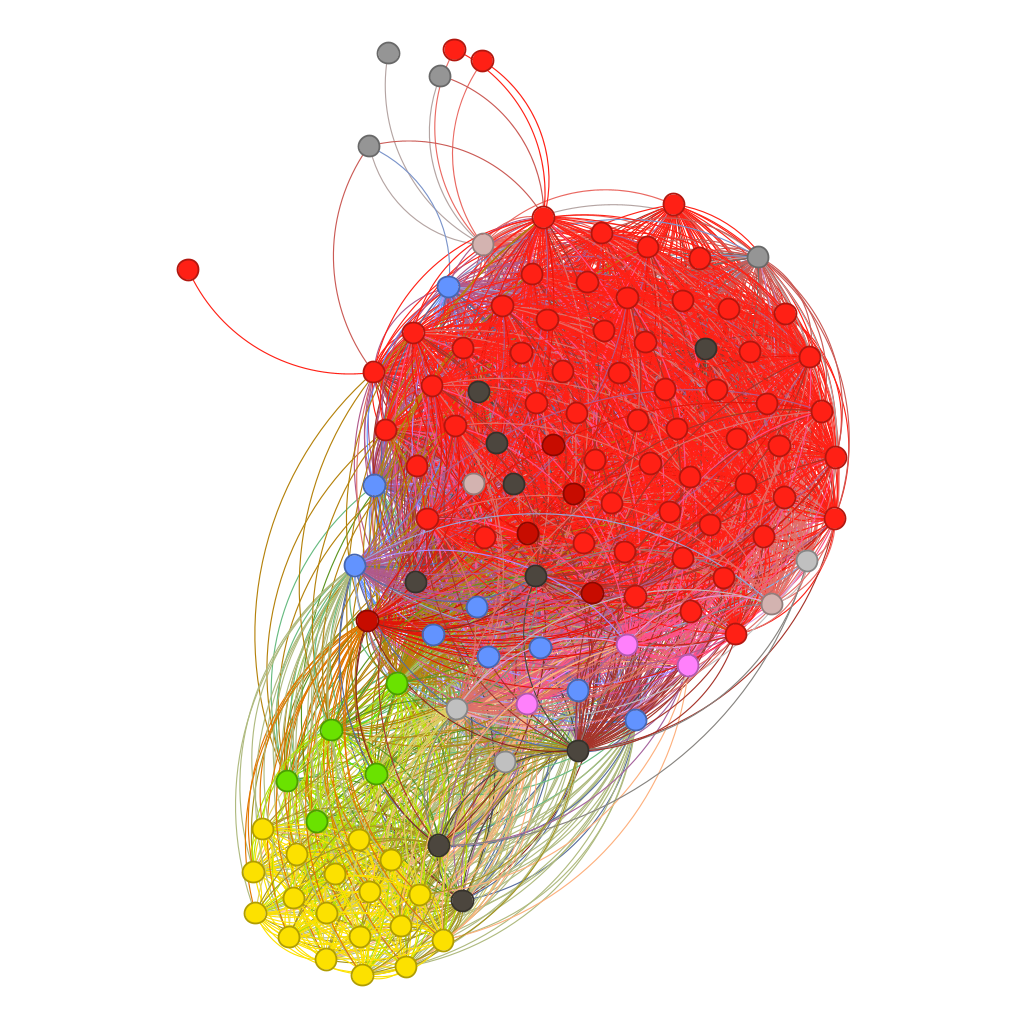
\includegraphics[width=\linewidth]{img/xvii_graph.png}
  \caption{Network of the XVII legislature. Different colors represent different political groups. Isolated nodes are not shown for visualization purposes.}
  \label{fig:graph}
\end{figure}


\begin{figure}[h]
  \centering
  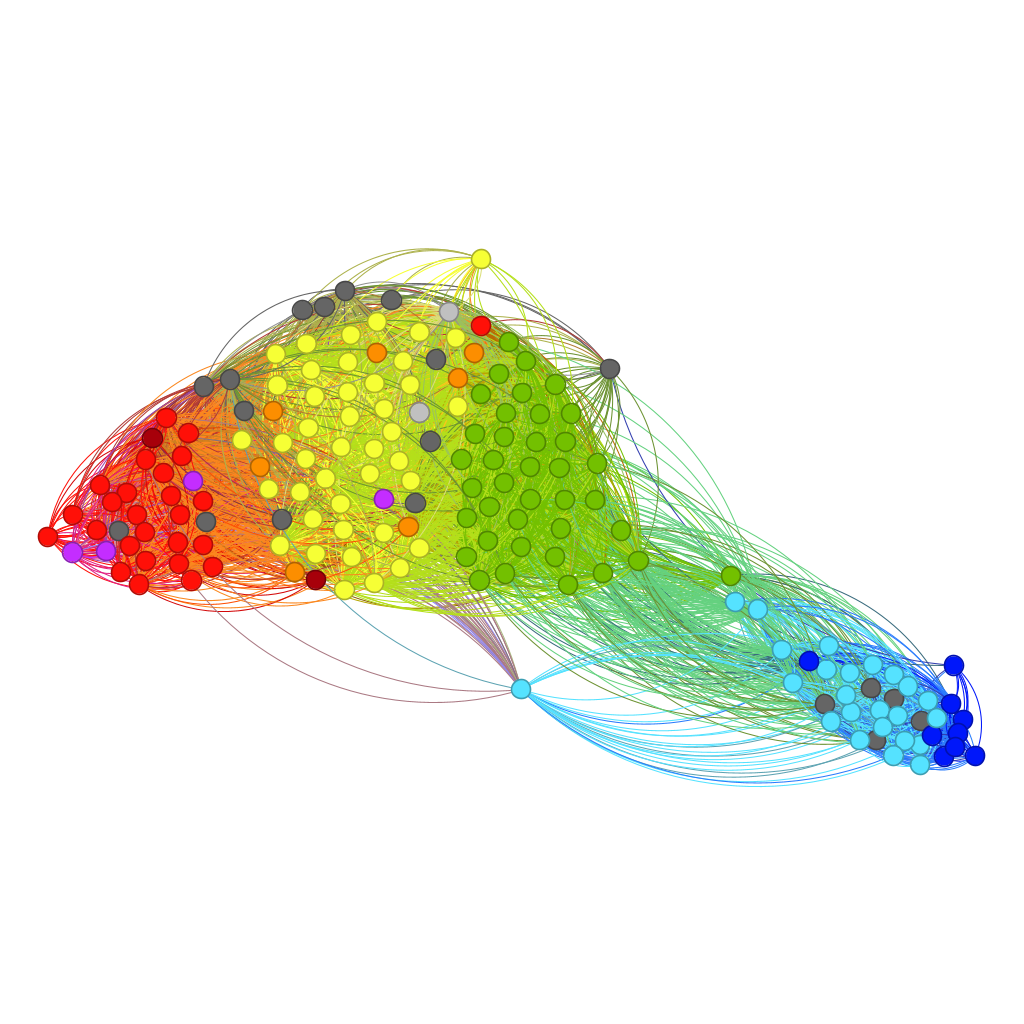
\includegraphics[width=\linewidth]{img/xviii_graph.png}
  \caption{Network of the XVIII legislature. Different colors represent different political groups. Isolated nodes are not shown for visualization purposes.}
  \label{fig:graph}
\end{figure}


In this section we will study the basic features of our network. For this purpose we will focus on aggregated data over a whole legislature. Nodes are represented by the deputies, and edges are built based on their voting similarity.\\
From now on, let's consider the XVII legislature.

\subsubsection{Nodes}
Applying the discussed preprocessing, we remain with 136 nodes in our network.

\subsubsection{Edge characterization}
Let's see more in detail how the edges were built.\\
The possible outcomes for each vote were:
\begin{enumerate}
    \item Absent
    \item In favour
    \item Against
    \item Abstention
\end{enumerate}
The nodes of our network are the members of the Chamber.\\
We introduce a weighted edge between each couple of Deputies.\\
\newpage

The weight is the similarity between their voting behaviors (excluding absence) defined as:
\begin{equation}
    \text{Similarity} = \dfrac{\text{\#same vote}}{\text{\#different vote + \#same vote}}
\end{equation}

Note that we only consider the votes in which both Deputies were present.
 We end up with a weighted graph.\\


\begin{figure}[h]
  \centering
  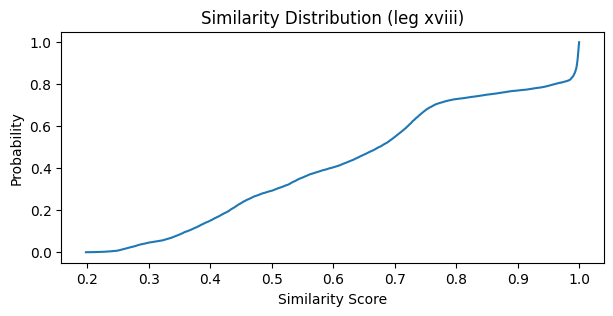
\includegraphics[width=\linewidth]{img/similarity_xvii.png}
  \caption{CDF for the similarity between nodes of the XVII legislature.}
  \label{fig:cdf}
\end{figure}

Now we want to introduce a threshold for the similarity and drop the edges which fall below it.
To define the threshold, let's consider the cumulative distribution function of the similarity (fig. \ref{fig:cdf}).
We decided to set our threshold in correspondence of the 50th percentile (median), considering only edges whose similarity value was above this value.\\
In the case of the XVII legislature,
 this corresponds to considering only edges with similarities above approximately 0.35.\\
Doing this, we pass from 9052
 to 4568 edges.


At this point, for simplicity, we drop the edge weights to work with an unweighted graph.\\

\subsection{Network Analysis}


Let's now analyze some basic features of our network: in table (\ref{tab:basic_measures}) we present an overview of the basic measures year by year.
It's important to note, that in the years $2015$ and $2016$ the networks are smaller, however, most of the metrics remain roughly stable throughout the years. The networks have all the same density more or less (by construction), and they have an extremely high average value of clustering coefficient. It's interesting to note that most of the networks have a single connected component.\\

As we said, from now on we focus on aggregated data of the XVII legislature.
\subsubsection{Degree distribution analysis} Let's now focus on the degree distribution of our network.
\begin{figure}[h]
  \centering
  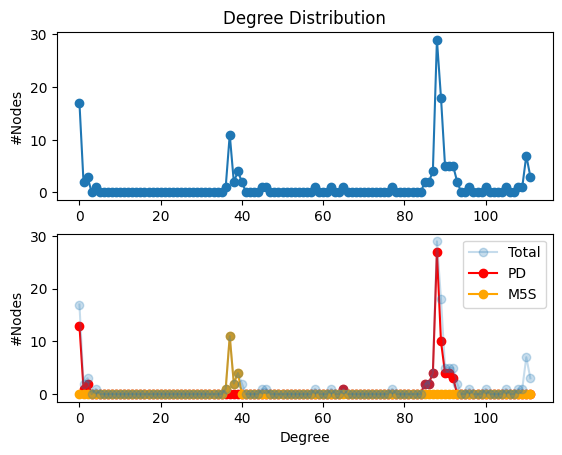
\includegraphics[width=\linewidth]{img/degree_xvii_party.png}
  \caption{Degree distribution of the network of the XVII legislature. In the bottom subplot, we consider the degree distributions separating members of the two main parties in the Chamber.}
  \label{fig:degree_distrib}
\end{figure}

Since we have a limited number of nodes, it is difficult to recognize a specific pattern.\\
If we look at figure (\ref{fig:degree_distrib}), apart from the peak at 0 (corresponding to 17 isolated nodes), we identify a peak around degree 40 and another around 90. These two peaks correspond to the two main political groups in the Chamber during the XVII legislature: M5S and PD. Their members, in general, voted similarly to the extent that also their degree is the same or nearly so.\\
The average degree is 67. Showing in general a high degree of connectivity.\\

In our analysis, as stated before, we set our edge threshold in correspondence with the median (in the case of the XVII legislature it corresponds to 0.35). However, it is interesting to study how the average degree changes if we change the edge threshold.
We can visualize that in figure (\ref{fig:degree_thresh}). Note that on the x axis we consider 50 linearly spaced thresholds from 0 to 1. 

\begin{figure}[h]
  \centering
  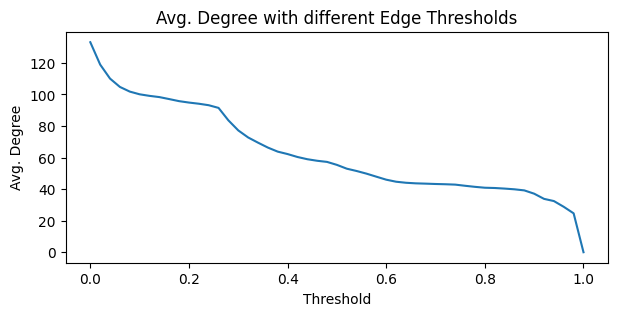
\includegraphics[width=\linewidth]{img/degree_xvii_varing_tresh.png}
  \caption{Average degree of the network of the XVII legislature, varying the applied edge threshold.}
  \label{fig:degree_thresh}
\end{figure}

As expected, increasing the threshold leads to a decreasing number of edges in the network. As an immediate consequence, the average degree decreases.

\subsubsection{Connected components analysis}

Excluding the isolated nodes (in this case 17), in the network we can identify a single connected component. It means that, with the selected threshold for similarity, bridges between different communities are maintained, and there is no complete segregation of parties.\\
Let's study how the situation changes varying the threshold, in figure (\ref{fig:conn_comps_thresh}).

\begin{figure}[h]
  \centering
  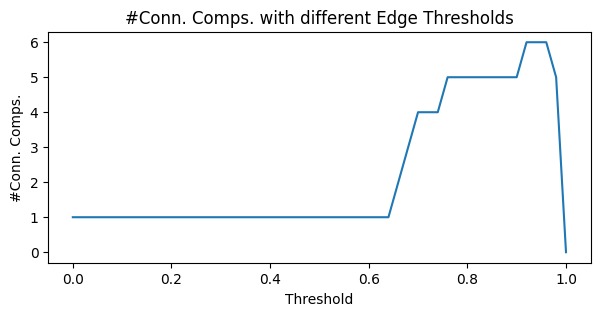
\includegraphics[width=\linewidth]{img/conn_comps_changing_thresh.png}
  \caption{Number of connected components of the network of the XVII legislature, varying the applied edge threshold.}
  \label{fig:conn_comps_thresh}
\end{figure}

We see that after a certain value (around 0.6) the number of connected components starts to increase. That is related to the decreasing number of edges in the network, that will eventually affect bridges between different connected components.

\subsubsection{Path analysis}
The average shortest path length is 1.37, while the network diameter is 3.
Both these measures display a densely connected graph.
The former measures the typical distance between pairs of nodes, and in this case it is rather small. The latter is a measure of the maximum number of edges needed to connect two nodes in the network. With a value of 3, it emphasize the dense nature of our network. 

\subsubsection{Clustering Coefficient, Density Analysis}

The average clustering coefficient is 0.80, while the density of the network is 0.50.\\
The average clustering coefficient provides insights into the connectivity of our network. It has a pretty high value, implying a general tendency to aggregation.\\
Note that the density is 0.50 by construction, since we decided to set the threshold for edges in correspondence of the median of the similarity.\\
In figure (\ref{fig:cc_dens_thresh}) we show how these properties change varying the threshold.\\

\begin{figure}[h]
  \centering
  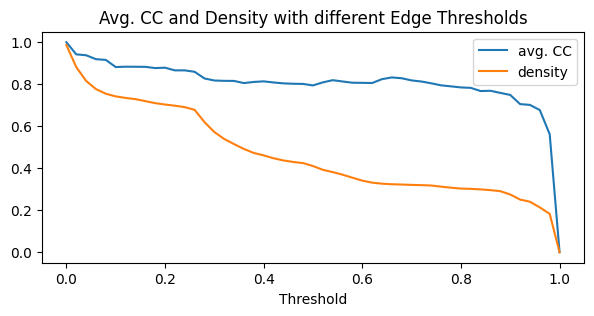
\includegraphics[width=\linewidth]{img/cc_density_xvii_varing_tresh.png}
  \caption{Average Clustering Coefficient and density of the network of the XVII legislature, varying the applied edge threshold.}
  \label{fig:cc_dens_thresh}
\end{figure}

We see that the average clustering coefficient is stable around 0.8-0.9 (except from when the threshold is 1 which means there are no edges in the graph). This means that the tendency to form local neighborhoods does not depend on the similarity threshold applied.\\
Of course, the density decreases while the threshold increases because we are removing more and more edges from the graph.

\subsubsection{Centrality analysis}
We now want to study some centrality properties of the network.\\
In particular we focus on Betweenness Centrality and Closeness Centrality of nodes, whose distributions are reported in figure (\ref{fig:centrality}).\\

Betweenness centrality is related to how much a node helps the network to remain connected. Since the network is pretty dense, values of betweenness centrality are all very close to 0.\\

Closeness centrality is related to the average distance between a node and all the other nodes in the network. Apart from isolated nodes (with CC = 0), we note that almost all nodes have a closeness centrality greater than 0.4, and most of them have values around 0.7. This shows that members of the Chamber are generally very close between them, in terms of voting behavior.
\begin{figure}[h]
  \centering
  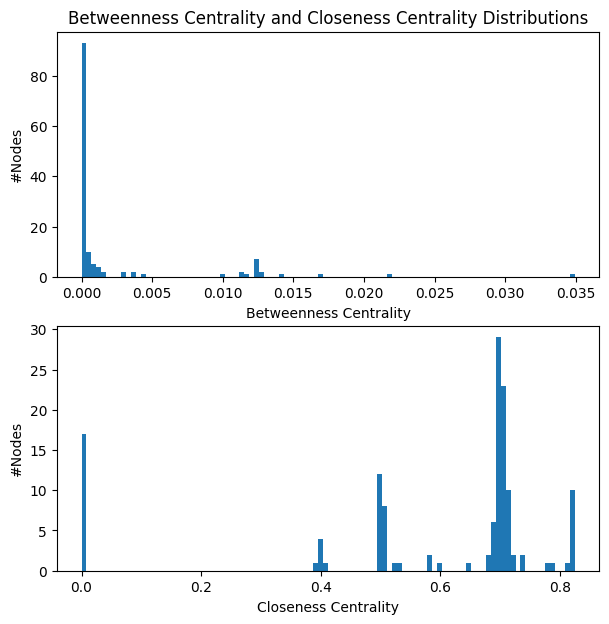
\includegraphics[width=\linewidth]{img/centrality_xvii.png}
  \caption{Betweenness Centrality (top) and Closeness Centrality (bottom) distributions for the network of the XVII legislature.}
  \label{fig:centrality}
\end{figure}

\subsection{Comparision with ER}
Let's now compare our graph with a random one.
To do that, we generate an ER graph with the same number of nodes as our graph, in our case 136. We also want our ER graph to have a similar number of edges to our real graph. To do so, we choose the value of p (probability of the presence of an edge between two nodes) according to the following relation:
\begin{equation}
    p = \dfrac{2 L}{N(N-1)}
\end{equation}
where N is the number of nodes and L is the number of edges.\\
In our case N = 136 and L = 4568, so we have p = 0.50. \\
In table (\ref{tab:er_ba}) we compare some of the basic measures computed on the ER graph, with the ones computed on our real network.
\begin{table}[h]
\begin{tabular}{lrrr}
\hline
               &    Real &      ER &      BA \\
\hline
 \#nodes        &  136 &  136 &  136 \\
 \#edges        & 4568  & 4570 & 4615 \\
 avg degree    &   67.18 &   67.21 &   67.87 \\
 \#isol. nodes  &   17 &    0 &    0 \\
 \#conn. comps. &    1 &    1 &    1 \\
 avg SPL       &    1.37 &    1.50 &    1.50 \\
 diameter      &    3 &    2 &    2 \\
 avg CC        &    0.80 &    0.50 &    0.72 \\
 Density       &    0.50 &    0.50 &    0.50 \\
\hline
\end{tabular}
\caption{Comparison of basic measures with ER and BA graphs.}
\label{tab:er_ba}
\end{table}

We note that the average degree of the ER graph is comparable to the one of our network. However, the degree distribution is pretty different, as we can see in figure (\ref{fig:degree_er}).

\begin{figure}[h]
  \centering
  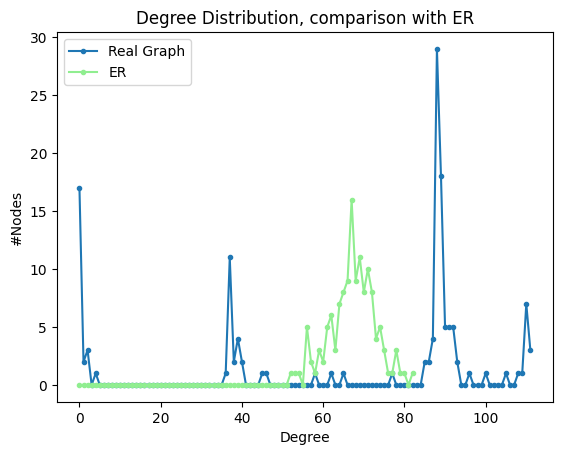
\includegraphics[width=\linewidth]{img/degree_dist_er_xvii.png}
  \caption{Degree Distribution: comparison between real graph and ER graph.}
  \label{fig:degree_er}
\end{figure}


The number of connected components, excluding isolated nodes, is the same. There is no significative difference in the average shortest path length either.\\
The diameter of the ER graph is 1 unit smaller than the real one; this is due to the fact that in the ER graph the connections are random, while in the real graph not all connections have the same probability to establish. For example, the path between two members of the Chamber with opposite political views will not be of length one, but will probably pass through one (or more) moderate member(s). This will make the network diameter wider with respect to the random scenario.\\

The average clustering coefficient of the random graph is significantly smaller than the one of the real graph. This highlights how the real network is, indeed, clustered.\\

Having almost the same number of edges, density is of course the same.


\subsection{Comparision with BA}

Finally, we compare our network with a Barabasi Albert graph. The BA graph is characterized by a scale-free topology with a power-law degree distribution. It is described by the (integer) parameter $m$, which determines the number of edges a new node forms with existing nodes during the growth process.\\
We chose for $m$ a value so that the number of edges of the BA graph was comparable with the number of edges of the real graph. In our case we have $m = 65$.\\

In table (\ref{tab:er_ba}) we compare some of the basic measures computed on the BA graph, with the ones computed on our real network, and on the ER graph.\\

We can see that the global properties of the BA network expressed in table (\ref{tab:er_ba}) are in line with the ones of the real graph. We note that the average SPL is slightly higher in the BA graph, and the average clustering coefficient is slightly smaller. This means that the level of clustering in our real network is, on average, greater than the scale-free case.\\
Finally, as we saw in the ER case, also in the BA graph the diameter is slightly smaller than the real case.\\

In figure (\ref{fig:degree_ba}) we plot the degree distribution of the BA graph compared with the real one. We see that the BA distribution does not capture the two peaks of the real one.\\

In conclusion, neither the ER model nor the BA model can capture the structure of the degree distribution of our network.

\begin{figure}[h]
  \centering
  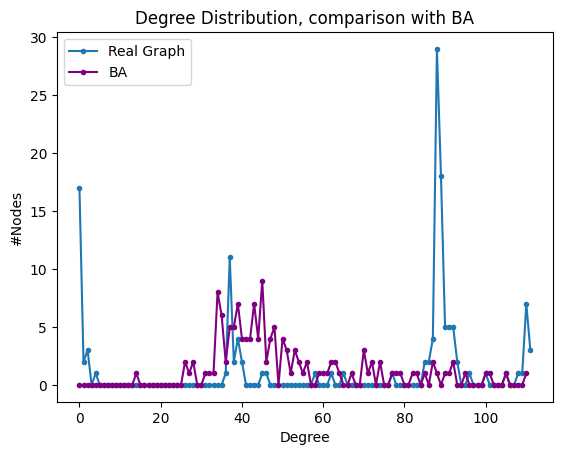
\includegraphics[width=\linewidth]{img/degree_dist_ba_xvii.png}
  \caption{Degree Distribution: comparison between real graph and BA graph.}
  \label{fig:degree_ba}
\end{figure}


%-----------------------

